\documentclass[a0paper,fontscale=0.3]{baposter}  % fontscale=0.285, dvipdfm

\usepackage{setspace}
\usepackage{multicol}
\usepackage{multirow}

\usepackage{amsmath}
\usepackage{algorithm}
\usepackage{algcompatible}
\usepackage[noend]{algpseudocode}
%\usepackage{tikz}
%\usepackage{pgfbaselayers}
%\pgfdeclarelayer{background}
%\pgfdeclarelayer{foreground}
%\pgfsetlayers{background,main,foreground}

%%% Color Definitions %%%%%%%%%%%%%%%%%%%%%%%%%%%%%%%%%%%%%%%%%%%%%%%%%%%%%%%%%

%\definecolor{bordercol}{RGB}{40,40,40}
%\definecolor{bordercol}{RGB}{100,0,0}
\definecolor{bordercol}{RGB}{0,0,0}
%\definecolor{headercol1}{RGB}{186,215,230}
%\definecolor{headercol2}{RGB}{80,80,80}
%\definecolor{headercol1}{RGB}{153,0,0}
%\definecolor{headercol2}{RGB}{153,0,0}
\definecolor{headercolone}{RGB}{6,130,22}
\definecolor{headercoltwo}{RGB}{6,130,22}
%\definecolor{boxcolor}{RGB}{186,215,230}
%\definecolor{boxcolor}{RGB}{110,230,209}
%\definecolor{boxcolor}{RGB}{143,255,236}
%\definecolor{boxcolor}{RGB}{171,255,241}
\definecolor{boxcolor}{RGB}{176,232,223}
\definecolor{headerfontcol}{RGB}{255,255,255}
%\definecolor{boxcolor}{RGB}{186,215,230}
%\definecolor{boxcolor}{RGB}{226,200,200}
%\newcommand{\hilitetwo}[1]{{\addfontfeature{Color=FF000099}#1}}
\newcommand{\hilitetwo}[1]{{\addfontfeature{Color=99333399}#1}}
%\newcommand{\hiliteone}[1]{{\addfontfeature{Color=33993399}#1}}
\newcommand{\hiliteone}[1]{{\addfontfeature{Color=06821699}#1}}
\newcommand{\hilitegrey}[1]{{\addfontfeature{Color=77777799}#1}}

%%% Utility functions %%%%%%%%%%%%%%%%%%%%%%%%%%%%%%%%%%%%%%%%%%%%%%%%%%%%%%%%%%

%%% Save space in lists. Use this after the opening of the list %%%%%%%%%%%%%%%%
\newcommand{\compresslist}{
        \setlength{\itemsep}{1pt}
        \setlength{\parskip}{0pt}
        \setlength{\parsep}{0pt}
}

\usepackage{polyglossia}
\setdefaultlanguage[variant=australian]{english}

\usepackage{expex}

\usepackage{fontspec}
\defaultfontfeatures{PunctuationSpace=3,Scale=MatchLowercase,Mapping=tex-text}
\newfontfeature{IPA}{+mgrk}
%\setromanfont[IPA]{FreeSerif}
%\setromanfont[IPA,Scale=0.8]{FreeSerif}
\setromanfont[IPA]{Liberation Serif}
%\setromanfont[IPA]{Times New Roman}
%\setromanfont[IPA]{NimbusRomNo9L-Regu}
%\setromanfont{Times New Roman}
%\setmonofont[IPA]{Liberation Mono}
\setmonofont[IPA]{DejaVu Sans Mono}
%\renewcommand{\sfdefault}{phv}
%\renewcommand{\rmdefault}{ptm}
%\renewcommand{\ttdefault}{pcr}
\usepackage[small,bf]{caption}
%\newfontfamily\qipa[IPA]{NimbusRomNo9L-Regu}
\newfontfamily\qipa[IPA,Scale=MatchLowercase]{FreeSerif}
\newfontfamily\qgmk[IPA,Scale=0.8]{FreeSerif}

\newfontfamily\litamono[IPA,Scale=0.5]{DejaVu Sans Mono}

\newcommand{\tilda}{{\qipa ∼}}

\newcommand{\tags}[1]{\hiliteone{#1}}
\newcommand{\newtag}[1]{\hilitegrey{<}\hiliteone{#1}\hilitegrey{>}}

%\newfontfamily\htwo[IPA,Scale=1.2]{FreeSans}}
%\newfontfamily\htwofont[IPA,Scale=1]{CMU Sans Serif}
%\newfontfamily\htwofont[IPA,Scale=1,Color=333344FF]{CMU Sans Serif}
\newfontfamily\htwofont[IPA,Scale=1,Color=111111FF]{FreeSerif}
%\newfontfamily\titlefont[IPA,Scale=0.52]{FreeSerif}
\newfontfamily\titlefont[IPA,Scale=0.7]{FreeSerif}
\newcommand{\htwo}[1]{{\htwofont \textbf{\dotfill{}#1\dotfill{}}}}
\usepackage{graphicx}  % [dvipdfm]

\definecolor{grey}{rgb}{0.91,0.91,0.91}
\newcommand{\codeex}[1]{
   \fbox{\colorbox{grey}{
         \begin{minipage}[t]{0.91\textwidth}{\litamono
            #1
         }\end{minipage}
      }
   }
}

\newcommand{\blank}[1]{\underline{\hspace{#1}}}
% FIXME: Breaks baposter
%\usepackage[novoc,fdf2alif]{arabxetex}
%\newfontfamily\uighurfont[Script=Arabic,Scale=1.5]{Lateef}
%\newfontfamily\arabicfont[Script=Arabic,Scale=1.5]{Lateef}

\usepackage{natbib}
\usepackage[colorlinks=true,citecolor=black,linkcolor=black,urlcolor=black]{hyperref}

\usepackage{subfigure}
\usepackage{booktabs}

%%\bibpunct{(}{)}{;}{A}{,}{,}
%\bibdata{paper}

\newcommand{\citemultileft}[1]{(\citeauthor{#1}, \citeyear{#1}}
\newcommand{\citemultimid}[1]{\citeauthor{#1}, \citeyear{#1}}
\newcommand{\citemultiright}[1]{\citeauthor{#1}, \citeyear{#1})}
\newcommand{\citetwoyears}[2]{\citeauthor{#1} (\citeyear{#1} and \citeyear{#2})}

% for glosses
\newcommand{\eng}[1]{`{\em #1}'}
%dammit, sc doesn't seem to be working
\newcommand{\gmk}[1]{{\qgmk \textsc{#1}}}


\usepackage{enumitem}
\setlist{nolistsep,leftmargin=*}
\newenvironment{itemise}[1]{
        \begin{itemize}\setlength{\leftmargin}{-4em}\setlength{\itemsep}{-0.2em}
        \vspace{-0.5em}
        #1
}{
        \end{itemize}
        \vspace{-2pt}
}

%\newcommand{\h2}[1]{{\big



\begin{document}
	% To get it to be A0 consistently on all machines..
	%\special{papersize=1189mm,841mm}
	\special{papersize=841mm,1189mm}
	\setlength{\pdfpageheight}{\paperheight}
	\setlength{\pdfpagewidth}{\paperwidth}

%%% Setting Background Image %%%%%%%%%%%%%%%%%%%%%%%%%%%%%%%%%%%%%%%%%%%%%%%%%%
%\background{
%	\includegraphics[width=0.99\textwidth]{flagkg2}
%}
	\background{{
	}}



	\begin{poster}{
			grid=false,
			%eyecatcher=false,
			borderColor=bordercol,
			headerColorOne=headercolone,
			headerColorTwo=headercoltwo,
			headerFontColor=white,
			% Only simple background color used, no shading, so boxColorTwo isn't necessary
			boxColorOne=boxcolor,
			headershape=roundedright,
  headerborder=open,
  headerheight=0.08\textheight,
  %headershape=roundedright,
  %headershade=plain,
  %headerfont=\Large\textsf, %Sans Serif
			%headerfont=\Large\sf\bf,
			textborder=rectangle,
			%background=plain,
			%background=user,
			background=none,
			headerborder=open,
			boxshade=plain,
			textborder=roundedleft,
		}{
			%\hspace{-2em}\includegraphics[height=6.5em,bb=0 0 242 203]{apertium}
			%\hspace{-2em}\includegraphics[height=6.5em,bb=0 0 612 792]{apertium2}
			%\hspace{-2em}\includegraphics[height=6.5em,bb=0 0 203 242]{apertium3}
			%\hspace{-2em}\includegraphics[height=6.5em,bb=0 0 242 203]{apertium3a}
			%\hspace{-2em}\includegraphics[height=6.5em,bb=0 0 242 203]{apertium4}
			\hspace{-2em}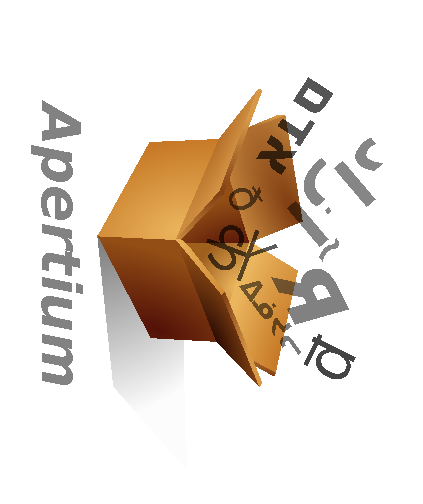
\includegraphics[angle=90,height=7.5em]{apertium5a}
			%Eye Catcher, empty if option eyecatcher=false - unused
		}{
			{\vspace{0pt}\hspace{-2.2ex}
			{\titlefont \textsc{Subsegmental language detection in Celtic language text}}}
		}{
			%Jonathan North Washington {\small (Indiana University, \texttt{jonwashi@indiana.edu})}, Mirlan Ipasov {\small (International Ataturk Alatoo University, \texttt{mipasov@gmail.com})}, Francis M.\ Tyers {\small (Universitat d'Alacant, \texttt{ftyers@dlsi.ua.es})}

			\vspace{-0.5em}
			\begin{center}
			{\begin{minipage}[t]{11.2em}
				\begin{spacing}{0.4}
					{Akshay Minocha}\\
					{\footnotesize IIIT Hyderabad\\Hyderabad, India\\\texttt{akshay.minocha@students.iiit.ac.in}}
				\end{spacing}
			\end{minipage}
			\begin{minipage}[t]{10.5em}
				\begin{spacing}{0.4}
					{Francis M.\ Tyers}\\
					{\footnotesize UiT Norgga Árktalaš Universitehta \\Romsa, Norway\\\texttt{francis.tyers@uit.no}}
				\end{spacing}
			\end{minipage}}
			\begin{minipage}[t]{5.5em}
				\vspace{-0.25em}
				\begin{spacing}{0.4}
					{\footnotesize Special thanks to}\\
					{\small Kevin Scannell}\\
					%{\footnotesize \texttt{sun27aida@gmail.com}}
					%{\small Ağarahim Sultanmuradov}\\
					%{\small A.\ Sultanmuradov}\\
					%{\small Google Summer of Code}\\
					%{\small Google Code-In}
					%{\small GSoC, GCI}
				\end{spacing}
			\end{minipage}
			\end{center}
		}{
			foo
		}
	\headerbox{Introduction}{name=kypchaklgs,column=0,row=0}{
		We aim to perform language identification on sub segmental basis: \\
		\begin{itemize}
			\item Typical case is to detect the language of documents and sentences. \\	
			\item We are focussing on cases where - A single sentence may have different code switching points \\
		\end{itemize}
                %\begin{figure}
		\begin{small}
		\begin{alltt}
		[\textbf{en} You're a] [\textbf{ga} Meirice\'{a}nach, c\'{e}n f\'{a}th] [\textbf{en} are you] [\textbf{ga} foghlaim Gaeilge?!] \\
		@afaltomkins [\textbf{cy} gorfod cael bach o tan] [\textbf{en} though init]	\\
		[\textbf{en} omg] [\textbf{cy} mar cwn bach yn] [\textbf{en} black and tan] [\textbf{cy} a popeth,] [\textbf{en} even cuter!!]
		\end{alltt}
		\end{small}
		%\caption{Example of text from a microblogging site chunked manually.}
		%\label{fig:tweets}
		%\end{figure}

	}
	
	\headerbox{Dataset}{name=morphtrans,below=kypchaklgs}{
		%\htwo{Morphological transducers}
		\begin{itemize}
			\item Simplifying the task by taking into account Celtic languages and a corresponding majority language. \\
			\item Manual annotation of about 40-50 tweets for each of the three language pairs.  \\
		\end{itemize}

		\begin{center}
		\begin{tabular}{|l|r|r|r|r}
		\hline
		\multirow{2}{*}{\textbf{Pair}} & \multirow{2}{*}{\textbf{Language}}  & \multicolumn{2}{c|}{\textbf{Statistics} (\%)} \\\cline{3-4}
		                &  &  Tokens & Segments \\
		\hline
		\multirow{2}{*}{Irish---English} & Irish & 332 & 40 \\
		                                 & English & 379 & 42 \\
		\hline
		\multirow{2}{*}{Welsh---English} & Welsh & 419 & 64 \\
		                                 & English & 378 & 66  \\
		\hline
		\multirow{2}{*}{Breton---French} & Breton & 388 & 54 \\
		                                 & French & 379 & 53  \\
		\hline
		\end{tabular}
		\end{center}
	%	\caption{Document statistics of the annotated data used. }
	%	\label{table:datastats}

	}

		\headerbox{Methodology}{name=exout,below=morphtrans}{

		\htwo{Alphabet n-gram approach}
		\newline
	   	\begin{itemize}
			\item	Character Language model
			\item	Using IRSTLM we build a language model for the five languages 
			\item	For English and French - Europarl 
			\item	Breton, Welsh and Irish - Corpora of text crawled from the web
			\item	Size of the corpus from which this language model was built - 1.5 million tokens
			\item 	Example - the word `sl\'{a}inte!' would be broken down into a sequence
of \{`\_ s', `s l', `l \'{a}', `\'{a} i', `i n', `n t', `t e', `e !', `! \_'\}.
		\newline
		\end{itemize}	

		\htwo{Word based prediction}
		\newline
		\begin{itemize}
			\item	Generate word lists for the languages using aspell which is widely used on Unix systems.
			\item 	Word are labeled according to their presence in the particular word list. 
			\item	In case of a confusion the word is added to the previous segment 
		\newline
		\end{itemize}
		\htwo{Word-based prediction with character backoff}
		\newline
		\begin{itemize}
			\item	Same as Word-based prediction, but in case of confusion this falls back to the Alphabet bi-gram approach. 
		\end{itemize}
		\htwo{Baseline}
		\newline
		\begin{itemize}
			\item	Using langid.py labeled all the lines in a particular dataset according to the majority classification 
		\newline
		\end{itemize}

		\htwo{Langid character trigram prediction}
		\newline
		\begin{itemize}
			\item	Trigram probabilities from langid were taken into account. 	
			\item	All other heuristics and chunking algorithm are same as for other methods.
		\newline
		\end{itemize}
		}


		\headerbox{Chunking algorithm}{name=lexc,column=1,row=0,span=2}{
		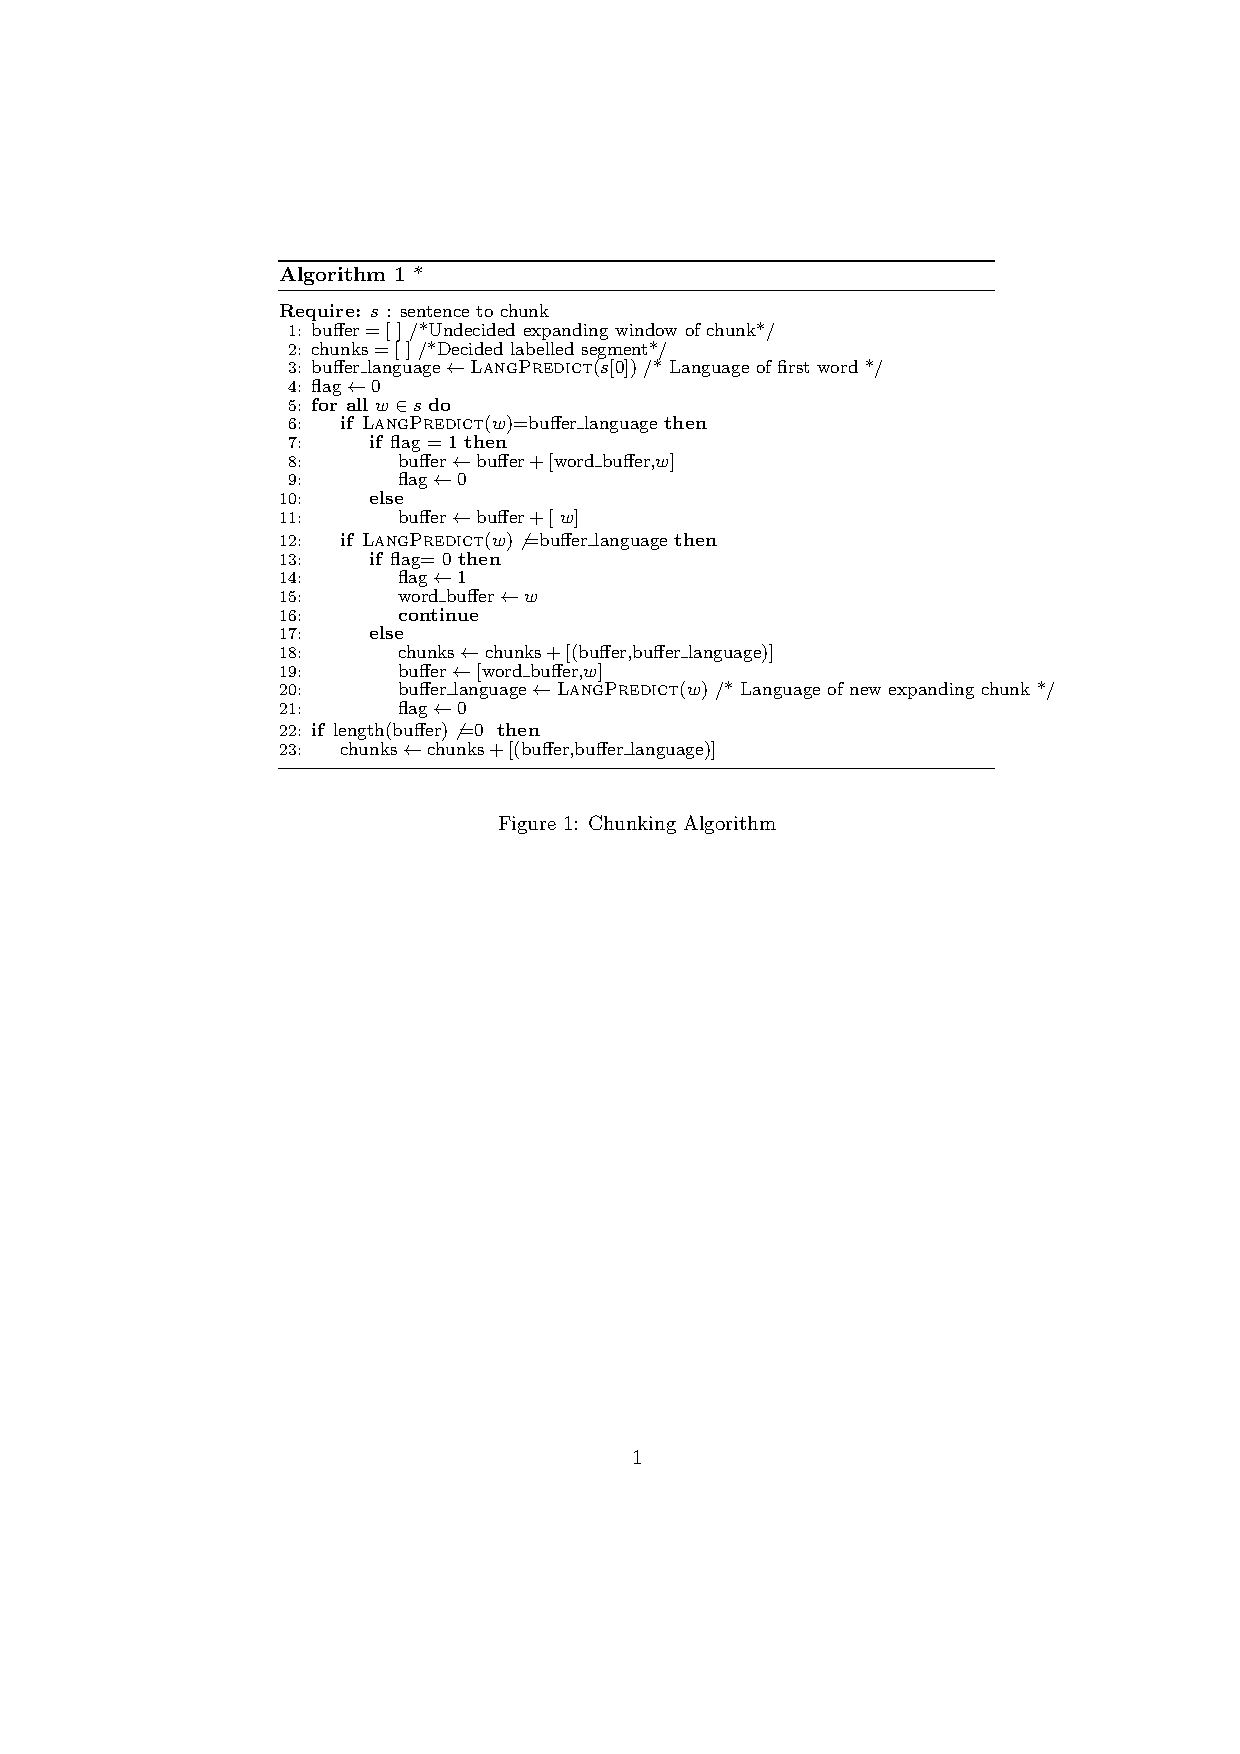
\includegraphics[trim = 4.4cm 10.5cm 0 4cm, clip, scale=0.55]{pseudocode.pdf}
%		\begin{algorithm}
%		\caption*{\textsc{}}
%		%\caption{Chunking algorithm}\label{euclid}
%		{\fontsize{9}{9}\selectfont
%		\begin{algorithmic}[1]
%		%\Statex{}%Procedure{}{}
%		\Require \(s\) : sentence to chunk
%		\State $\textrm{buffer} = [\ ] \text{ /*Undecided expanding window of chunk*/}$
%		\State $\textrm{chunks} = [\ ] \text{ /*Decided labelled segment*/ }$
%		\State $\textrm{buffer\_language} \gets \textsc{LangPredict}(s[0]) \text{ /* Language of first word */ }$
%		\State $\textrm{flag} \gets \text{0}$
%		%\State $\text{for \ } \textit{word \ } \text{in \ } \textit{sentence:} $
%		\ForAll{\(w \in s\)} %{\texttt{word in sentence}}
%		\If {$ \textsc{LangPredict}(w) \text{=} \textrm{buffer\_language} $}
%		        \If {$ \textrm{flag} \text{\ = 1} $}
%		        \State $\textrm{buffer} \gets \textrm{buffer} + [\textrm{word\_buffer,\(w\)}] $
%		        \State $\textrm{flag} \gets \text{0}$
%		        \Else
%		        \State $\textrm{buffer} \gets \textrm{buffer} +[\textrm{ \(w\)}] $
%		        \EndIf
%		        \EndIf
%		\If {$ \textsc{LangPredict}(w) \not{=} \textrm{buffer\_language} $}
%		        \If {$ \textrm{flag} \text{=\ 0} $}
%		        \State $\textrm{flag} \gets \text{1}$
%		        \State $\textrm{word\_buffer} \gets \textrm{\(w\)} $
%		        \State $\textbf{continue}$
%
%		        \Else
%		        \State $\textrm{chunks} \gets \textrm{chunks} + \textrm{[(buffer,buffer\_language)]} $
%		        %\State $\textit{buffer} \gets [] $
%		        \State $\textrm{buffer} \gets [\textrm{word\_buffer,\(w\)}] $
%		        \State $\textrm{buffer\_language} \gets \textsc{LangPredict}\text{(\(w\))} \text{ /* Language of new expanding chunk */}$
%		        \State $\textrm{flag} \gets \text{0}$
%		        \EndIf
%	
%		\EndIf
%		\EndFor
%		\If {$\textrm{length(buffer)} \not{=} 0\ $}
%		        \State $\textrm{chunks} \gets \textrm{chunks} +[\textrm{(buffer,buffer\_language)}] $
%		
%		\EndIf
%		\end{algorithmic}}
%		\end{algorithm}
%		\vspace{-0.4cm}
%		\begin{figure}[hb]
%		\def\@fs@post{}
%		\caption{Chunking Algorithm}
%		\label{fig:chunkal}
%		\end{figure}
			}

					\renewcommand{\arraystretch}{0.65}



		
		\headerbox{Results}{name=results,column=1,row=1,span=2,below=lexc}{
			
			\begin{center}
			\begin{tabular}{|lc|r|r|r|r|r|r|}
			\hline
			\multirow{2}{*}{\textbf{System}}            & & \multicolumn{2}{c}{\textbf{Irish---English}} & \multicolumn{2}{|c|}{\textbf{Welsh---English}} & \multicolumn{2}{c|}{\textbf{Breton---French}}  \\\cline{3-8}
			                                          &      &  Irish &  English & Welsh  & English & Breton & French \\
			\hline
			\multirow{2}{*}{\texttt{baseline}}        &  $p$ &  2.50   & 0.0      & 0.0   & 0.0 & 0.0 & 0.0 \\
			                                          & $r$  & 2.56    & 0.0      & 0.0   & 0.0 & 0.0 & 0.0 \\
			\hline
			\multirow{2}{*}{\texttt{langid-3character}}         &  $p$ &  5.00   & 14.29    & 0.0   & 21.21 & 1.85 & 20.75 \\
			                                          & $r$  & 5.41    & 8.45     & 0.0   & 14.58 & 1.92 & 12.36 \\
			\hline
			\multirow{2}{*}{\texttt{wordlist}}        &  $p$ &  32.50 & 28.57     & 26.69 & {\bf 40.91} & 57.41 & 33.96 \\
			                                          & $r$  & 23.64  & 26.09     & {\bf 26.03} & {\bf 33.75} & 47.69 & 33.33 \\
			\hline
			\multirow{2}{*}{\texttt{character bigram}}          &  $p$ &  32.50   & 35.71   & 23.44 & 19.70  & 57.41 & 52.83 \\
			                                          & $r$  & 22.41    & 26.79   & 15.31 & 16.67 & 41.33 & 37.84 \\
			\hline
			\multirow{2}{*}{\texttt{wordlist+character bigram}} &  $p$ &  {\bf 52.50}   & {\bf 50.00}   & {\bf 32.81} & 31.82 & {\bf 70.37} & {\bf 67.92} \\
			                                          & $r$  & {\bf 38.18}    & {\bf 43.75}   & 24.14 & 25.61 & {\bf 57.58} & {\bf 57.14} \\
			\hline
			\end{tabular}
			\end{center}
			\vspace{-0.4cm}
		\caption{Precision, $p$ and recall, $r$ for the systems by language.}
			\label{table:precisionrecall}
			

			\begin{center}
			\begin{tabular}{|l|r|r|r|}
			\hline
			\multirow{2}{*}{\textbf{System}} &  \multicolumn{3}{c|}{\textbf{Accuracy} (\%)} \\\cline{2-4}
			       &   Irish---English & Welsh---English & Breton---French \\
			\hline
			\texttt{baseline} & 42.76 & 42.16 & 44.07 \\
			\hline
			\texttt{langid-3character} & 57.24 & 45.92 & 43.16 \\
			\hline
			\texttt{wordlist} & 79.75 & \textbf{74.28} & 83.96 \\
			\hline
			\texttt{character bigram} & 81.29 & 65.62 & 76.79 \\
			\hline
			\texttt{wordlist+character bigram} & \textbf{85.79} & 72.40 & \textbf{88.79} \\
			\hline
			\end{tabular}
			\end{center}
			\vspace{-0.4cm}
		\caption{Accuracy of the systems over the three language pairs. The accuracy measures how often a token
			  was assigned to the right language, independent of span.}
			\label{table:accuracy}

}
		\headerbox{Evaluation}{name=eval,column=1,below=results}{
		\begin{itemize}
		\newline	
			\item	We followed the footsteps of CoNLL 2000 shared task on language independent named entity recognition. 
		\newline	
			\item	Divide the text into non-overlapping segments.
		\newline	
			\item	Precision - percentage of correctly detected phrases.
		\newline	
			\item	Recall - number of phrases in the data that were found by the chunker.
		\newline	
		\end{itemize}
		}
		

		\headerbox{Conclusions}{name=conclusions,column=2,below=results}{
			\begin{itemize}
			\item	A very preliminary investigation into subsegment language identification in Celtic language texts.
		\newline	

			\item	We would like to include supervised methods and features talked about by King and Abney (2013)
		\newline	

			\item	We would also like to check our methods with higher order n-grams and more options in backoff.
		\newline	

			\item	Explore a lattice technique where each word is a lattice node and the inclusions of the words are done using probability.
		\newline	
			\end{itemize}
		}

\end{poster}
\end{document}
